% +---------------------------------------------------------------------------+
% | CGAL Reference Manual:  visibility_complex.tex
% +---------------------------------------------------------------------------+
% | Visibility complex. Implemented by topological sweep using the 
% | Greedy Flip Algorithm
% |
% | 21.01.2001   Pierre Angelier and Michel Pocchiola
% |              
% | 
\RCSdef{\vcomplexRev}{$Revision$}
\RCSdefDate{\vcomplexDate}{$Date$}
% +---------------------------------------------------------------------------+

\ccParDims

\chapter{Visibility Complexes}
\label{chapterVisibilityComplex}
\ccChapterRelease{\vcomplexRev. \ \vcomplexDate}\\
\ccChapterAuthor{Pierre Angelier and Michel Pocchiola}

\minitoc

% +----------------------------------------------------------------------------+
\section{Introduction}
\label{sectionVComplexIntroduction}
This package implements the visibility complex structure introduced by Pocchiola
and Vegter in~\cite{pv-vc-96} (see also~\cite{pv-tsvcpt-96}
and~\cite{G-ap-sstvc-01} for a more recent presentation). Although a
generalization to three dimensional environments has been proposed
in~\cite{ddp-fahrgv-99} we deal here only with planar scenes. 

The visibility complex is a 2D cell complex whose 1-skeleton is isomorphic to
the visibility graph.  The visibility graph can be used to compute the shortest
path between two points in a planar scene. A survey on visibility graphs and
shortest paths can be found in~\cite{m-gspno-00}.

Our implementation of the visibility complex structure follows closely the
design of the \ccc{Halfedge Data Structure} (see the introduction in
Chapter~\ref{chapterHalfedgeDS} and~\cite{k-ugpdd-99}) however this chapter can
be understood without reading the corresponding chapter.

We use the so-called Greedy Flip Algorithm (again see~\cite{pv-tsvcpt-96}) to
compute the visibility complex in optimal time complexity $O(k + n\log n)$ where
$n$ is the size of the input and $k$ the size of the output (i.e. the visibility
complex).
% +----------------------------------------------------------------------------+
\section{Definitions}
In this section we review the basic concepts defined in~\cite{G-ap-sstvc-01}
which are useful to understand the basic functionality of the package.

\paragraph{Basic definitions. }
A \emph{disk} is a bounded closed convex subset of the plane and a \emph{scene}
is a collection of pairwise disjoint disks. For the ease of the exposition we
will assume that the disks have non-empty interior and that the tangent line at
a point on the boundary of a disk is well defined. We will also suppose that our
disks are in general position that is, that there is no line tangent to three
disks. Although these definitions rule out points, segment and polygons our
implementation can handle these types of disks through a symbolic perturbation
scheme which is invisible to the user.  The general position assumption is also
lifted through perturbation.  More details are given in the degeneracies section
below. Note also that non convex polygons are also supported via the use of
\emph{constraints} which are defined further on.

A \emph{bitangent} is a directed line segment tangent to two disks and
intersecting these disks only at its endpoints.  The disk containing the source
and target point of the bitangent are called respectively the source and target
disk.  Two disks share four bitangents directed from the first towards the
second. 

\begin{ccTexOnly}
    %\vspace{-7mm}
    \begin{center}
      \parbox{0.4\textwidth}{%
          \includegraphics[width=0.4\textwidth]{fig/bitangent.eps}%
      }
    \end{center}
    %\vspace{-5mm}
\end{ccTexOnly}

\begin{ccHtmlOnly}
    <CENTER>
        <img src="fig/bitangent.gif" alt="Bitangent"><P>
    </CENTER>
\end{ccHtmlOnly}

The \emph{type} of a bitangent $t$ directed from a disk $A$ to a disk $B$ codes
the positions of $A$ and $B$ with respect to the supporting line of $t$. As
illustrated in the Figure above there are four possible types called \texttt{LL,
RR, LR} and \texttt{RL}. A \texttt{LR} bitangent $t$ for example, is such that
$A$ and $B$ lie respectively on the left and on the right of the supporting line
of $t$. 

Consider a scene $S$. A bitangent between two disks of $S$ is \emph{free} if its
interior does not intersect a disk of $S$.  A \emph{constrained scene} $S_H$ is
a scene $S$ and a subset $H$ of pairwise non crossing free bitangents. The
bitangents of $H$ are called \emph{constraints}. A bitangent is \emph{free} in
$S_H$ if it is free in $S$ and does not intersect a bitangent of $H$.
Constraints are still called free bitangents of $S_H$.

The set of free bitangents tangent to a given disk partition its boundary into
what we call \emph{arcs}. In other words an arc is a portion of the boundary of
a disk defined by two consecutively tangent bitangents.

A \emph{positive arc} belonging to a disk $d$ is an arc whose tangent lines leave 
$d$ on its left. The definition of a \emph{negative arc} is obtained by
replacing the word "left" with "right". Thus for each arc we consider two
copies of it: a positive and a negative one. A \emph{signed arc} is a positive
or a negative arc.

\paragraph{Visibility graphs. }
Given a constraint scene $S_H$, the \emph{visibility graph} of $S_H$ is the
directed graph where there is:
\begin{itemize}
    \item one vertex per free bitangent of $S_H$.
    \item one edge per signed arc. The edge connects the two vertices
    corresponding to the bitangents defining the arc. A counter-clockwise
    orientation of the boundary of the disks induce an orientation of the edges
    of the visibility graph.
\end{itemize}
Let $e$ be an edge. The two vertices connected by $e$ are denoted $\inf(e)$ and
$\sup(e)$ and are called the source and sink of $e$. These vertices are such
that $e$ is directed from $\inf(e)$ towards $\sup(e)$.

Each vertex of the visibility graph is incident to four edges (two on the source
disk and two on the target disk). The names of these edges are given in the
Figure below.
\begin{ccTexOnly}
    \begin{center}
	\psfrag{v}{$v$}
	\psfrag{ccw_target_edge(v)}{\texttt{ccw\_target\_edge}($v$)}
	\psfrag{cw_target_edge(v)}{\texttt{cw\_target\_edge}($v$)}
	\psfrag{ccw_source_edge(v)}{\texttt{ccw\_source\_edge}($v$)}
	\psfrag{cw_source_edge(v)}{\texttt{cw\_source\_edge}($v$)}
	\psfrag{e}{$e$}
	\psfrag{sup(e)}{$\sup(e)$}
	\psfrag{inf(e)}{$\inf(e)$}
	\includegraphics[height=8cm]{fig/edge-vertex.eps}%
    \end{center}
\end{ccTexOnly}

\begin{ccHtmlOnly}
    <CENTER>
	<img src="fig/edge-vertex.gif" alt="Edge-Vertex adjacencies"><P>
    </CENTER>
\end{ccHtmlOnly}

\paragraph{Visibility complexes. }
For more sophisticated visibility queries, the visibility complex is more
appropriate than the visibility graph. It has a richer two-dimensional cell
structure whose 1-skeleton (i.e. the graph obtained by keeping only the
vertex/edges incidences) is exactly the visibility graph. The definition of the
visibility complex is more tricky and requires the reader to be familiar with
the concepts of \emph{equivalence classes}, \emph{quotient space} and the
\emph{cutting} of a surface along a curve. The rest of the definitions of this
section can be skipped if one plans to use only the functionality of the
visibility graph (shortest paths for example).

Consider a constrained scene $S_H$. The \emph{free space} of $S_H$ is the
space obtained by cutting the complement of the interior of the disks of $S$
along the constraints of $H$.

A \emph{ray} is a pair $(p,\alpha)$ consisting of a point $p$ in free space and
a direction $\alpha \in \mathbb{S}^1$ (the 1-sphere).  The \emph{visibility
complex} of a constrained scene $S_H$ is the quotient space of the set of rays
with respect to the following equivalence relation $\sim$:
\begin{equation}
(p,\alpha) \sim (q,\beta) \textrm{ iff. } \alpha = \beta \textrm{ is the
direction of the line $(p,q)$ and the segment } [p,q] \textrm{ lies in the free
space of } S_H.
\end{equation}
The origins of the rays belonging to a same equivalence class define a maximal
length segment in free space or \emph{maximal segment} for short.  The
visibility complex is a two dimensional cell complex. We describe its elements
in the case where the set of constraints is empty. The adjunction of constraints
is discussed later on. The 0,1 and 2-dimensional cells of the visibility complex
are respectively:
\begin{itemize}
    \item \emph{Vertices}: a vertex corresponds to a maximal segment tangent to
    two disks. Each vertex has its associated geometric bitangent.
    \item \emph{Edges}: an edge corresponds to maximal segments tangent to one
    disk and touching the same pair of disks at their extremities. \\
    Let $e$ be an edge corresponding to maximal segments tangent to a disk $o$.
    If $o$ lies on the left of the supporting line of these segments then $e$ is
    said to be \emph{positive}. Otherwise $e$ is \emph{negative}.
    \item \emph{Faces}: a face is the set of maximal segments that touch the
    same pair of disks. The disk containing the source (resp. the target) of 
    these maximal segments is called the backward view (resp. forward view) of 
    the face.
\end{itemize}

\begin{ccTexOnly}
    \begin{center}
	\psfrag{Vertices}{Vertices}
	\psfrag{Edge}{Edge}
	\psfrag{Face}{Face}
	\psfrag{forward view}{forward view}
	\psfrag{backward view}{backward view}
	\includegraphics[height=5cm,width=\linewidth]{fig/vis-complex.eps}%
    \end{center}
\end{ccTexOnly}

\begin{ccHtmlOnly}
    <CENTER>
        <img src="fig/vis-complex.gif" width="90%" 
	 alt="The cells of the Visibility Complex"><P>
    </CENTER>
\end{ccHtmlOnly}

The 1-skeleton of the visibility complex is isomorphic to the visibility graph.
The additional information brought by the visibility complex resides in the
faces. Each maximal segment defines an unique face.

We now describe the different incidences between vertices, edges and faces in
the visibility complex. The discussion below is valid for scene that do not
contain constraints. The adjunction of these involves a small change concerning
edges which is discussed later on.
\begin{itemize}
    \item \emph{Face - Vertex incidences. } The number of vertices adjacent to a
    given face $\sigma$ is at least $2$ and at most linear. We offer an access
    to two vertices of particular interest denoted by $\sup(\sigma)$ and 
    $\inf(\sigma)$ which are intuitively the segments in the face with maximal 
    and minimal angle. More precisely the set of maximal segments of a face is
    ordered by the following relation:
    \begin{equation}
		    a < b \textrm{ iff. } \det(a,b) > 0.
    \end{equation}
    The vertices $\inf(\sigma)$ and $\sup(\sigma)$ are respectively the minimum
    and maximum for this order. \emph{Warning: convex-hull vertices...}\\
    Each vertex $v$ is incident to six faces. 
    \item \emph{Edge - Face incidences. } An edge $e$ is adjacent to three
    faces. These are obtained by taking a maximal segment of the edge and moving
    it slightly. See the figure below for the names of these faces.

    \begin{ccTexOnly}
	\begin{center}
	    \psfrag{dl(e)}{dl($e$)}
	    \psfrag{dr(e)}{dr($e$)}
	    \psfrag{ul(e)}{ul($e$)}
	    \psfrag{ur(e)}{ur($e$)}
	    \psfrag{e}{$e$}
	    \psfrag{Positive edge}{Positive edge}
	    \psfrag{Negative edge}{Negative edge}
	    \includegraphics[height=5cm,width=\linewidth]{fig/edge-face.eps}%
	\end{center}
    \end{ccTexOnly}

    \begin{ccHtmlOnly}
	<CENTER>
	    <img src="fig/edge-face.gif" width="90%"
	     alt="Edge-Face adjacencies"><P>
	</CENTER>
    \end{ccHtmlOnly}
    For a positive edge $e$ we set dr$(e) = $dl$(e)$ and for a negative edge
    ur$(e) = $ul$(e)$.
    \item \emph{Edge - Vertex incidences. } These incidences were described in
    the Visibility Graph section above.
\end{itemize}

We now describe the two main differences brought by the adjunction of
constraints (a more detailed and complete discussion can be found
in~\cite{G-ap-sstvc-01}).  First, the vertices corresponding to constraints are
adjacent to $8$ faces rather than $6$ before. The other difference is that the
visibility complex also contains special types of edges arousing from rays
emanating from the extremity of a constraint. Such an edge $e$ is called a
\emph{constraint edge} and is adjacent to only one face denoted by face$(e)$.
See the Figure below for an illustration.
\begin{ccTexOnly}
    \begin{center}
	\psfrag{face(e)}{face($e$)}
	\psfrag{e}{$e$}
	\psfrag{constraint}{constraint}
	\includegraphics[height=5cm]{fig/constraint-edge.eps}%
    \end{center}
\end{ccTexOnly}

\begin{ccHtmlOnly}
    <CENTER>
	<img src="fig/constraint-edge.gif" alt="Constraint Edges"><P>
    </CENTER>
\end{ccHtmlOnly}

\paragraph{Visibility complex antichains. } The antichain is an advanced feature
for users wishing to take advantage of the linear storage of the Greedy Flip
Algorithm which we have implemented to compute the visibility complex. In this
section we will only give an intuitive definition of the antichain. More details
can be found in~\cite{pv-tsvcpt-96}. 

The Greedy Flip Algorithm, or \textsc{Gfa} for short, is a topological sweep
algorithm.  To keep the description on the intuitive side imagine the visibility
complex embedded in $\mathbb{R}^3$. The \textsc{Gfa} sweeps the complex using a
plane.  The set of faces and edges intersected by this plane is what we call the
antichain.

We have added an iterator interface to greatly ease the use of the antichain.
The small piece of code below reads a list of segments from a file and outputs
the vertices of the visibility complex in optimal time and $O(n)$ storage.

\ccIncludeExampleCode{Visibility_complex/example1.C}

The antichain is closely connected to so-called greedy pseudo-triangulations.
This is illustrated in an example below but bare in mind that this package does
not aim to provide a convivial interface to pseudo-triangulations. An extension
package concerning pseudo-triangulations should appear in the future. The
interested user is invited to contact the authors.

\paragraph{Degenerate cases.} The above discussion holds for disks which have
non empty interior and a smooth boundary. However, our implementation can handle
points, segments and convex polygons which are what we call degenerate cases. 
This is achieved via a symbolic perturbation obtained by taking the Minkowski sum 
of a degenerate disk with a small circle having an infinitesimal radius. 

\begin{ccTexOnly}
    \begin{center}
	\includegraphics[height=4cm]{fig/perturbation.eps}%
    \end{center}
\end{ccTexOnly}

\begin{ccHtmlOnly}
    <CENTER>
        <img src="fig/perturbation.gif" alt="Perturbation"><P>
    </CENTER>
\end{ccHtmlOnly}

This perturbation implies no numerical computations and is completely
invisible to the user. Each time a scene contains a degenerate disk, the user
is invited to mentally replace it by its perturbated version in order to
visualize the visibility complex or graph. 

\begin{ccTexOnly}
    \begin{center}
	\psfrag{Perturbation}{Perturbation}
	\includegraphics[height=4cm]{fig/points.eps}%
    \end{center}
\end{ccTexOnly}

\begin{ccHtmlOnly}
    <CENTER>
        <img src="fig/points.gif" alt="Points"><P>
    </CENTER>
\end{ccHtmlOnly}

As an example, consider two points as in the figure above. They share four
bitangents which are geometrically equal. These four bitangent are nevertheless
represented by four different vertices in the visibility graph. The order of the
tangent points of these bitangents on the "boundary" of the point is determined
by the order of these tangent points if the points were replaced by small
circles. Considering the crossing predicate, the \texttt{LR} and \texttt{RL}
bitangents is the only crossing pair in the figure above.  Also bear in mind
that the presence of degenerate cases may imply arcs with zero length.

Finally we explain how the general position assumption is dealt with.
\emph{A finir ...}

\paragraph{General polygonal configurations. } Recall that disks, as they are defined
above, are convex. We now describe how to treat not only non convex polygons but
also more general polygonal configurations. Consider the general setting consisting in a 
family $S$ of pairwise non crossing segments which are allowed to share an
extremity. The set $S$ can for example be the edges of a non-convex polygon.
We use the following recipe to build a scene $T$ respecting our requirements:
\begin{itemize}
    \item Each extremity of a segment in $S$ is inserted as a point in $T$.
    Recall that points are treated symbolically as if they were small circles
    (see the paragraph above concerning degenerate cases). 
    \item Each segment $s \in S$ directed from point $p$ to point $q$, with $p,q
    \in T$ is inserted in $T$ as a constraint directed from $p$ to $q$. The type
    chosen for the constraint (recall that four types are possible) is
    \texttt{RL}. The reason for this choice is to avoid two crossing constraints.
\end{itemize}

The Figure below shows a polygonal configuration $S$ and the scene $T$ which
has to be given as an input to our algorithms. 

\begin{ccTexOnly}
    \begin{center}
	\psfrag{S}{$S$}
	\includegraphics[height=8cm]{fig/configuration.eps}%
    \end{center}
\end{ccTexOnly}

\begin{ccHtmlOnly}
    <CENTER>
        <img src="fig/configuration.gif" alt="Polygonal configurations"><P>
    </CENTER>
\end{ccHtmlOnly}

The aim of the \ccc{Visibility_complex_scene} class is to make the above recipe
more transparent. In fact, one can blindly use this class to compute visibility
complexes of polygonal configurations without understanding the above
discussion. The code below illustrates the use of this class.

\ccIncludeExampleCode{Visibility_complex/example2.C}

\paragraph{Output / Partial order. } 
\label{sectionVComplexInputOutput}
The vertices of the visibility complex are
accessed in our implementation via an iterator pair \texttt{vertices\_begin(),
vertices\_end()}. We now describe how these vertices are ordered. A natural idea
would be an order based on the angle of the bitangent with respect to a
horizontal direction. Unfortunately obtaining such an order would require at
least $O(k \log n)$ in time complexity, where $k$ is the size of the output and
$n$ the size of the input. Since we achieve an optimal bound of $O(k + n\log
n)$, our order is slightly more subtle than an angle-based order. It is a linear
extension of a partial order $\prec$. In other words if $a \prec b$  then $a$
appears before $b$. Moreover the partial order is compatible with angle-order:
if $a \prec b$ then the angle of $a$ with respect to a horizontal direction is
smaller than the angle of $b$. The converse is \emph{not} necessarily true.

Let $S_H$ be a constrained scene containing $n$ disks; we define the partial
order $\prec$ as the transitive closure of $2n$ total orders (two per disk). \\
Let $B_o$ be the set of free bitangents tangent to $o$ and such that $o$ lies
on the half-plane to the left of their supporting lines. The angle of a
bitangent with respect to a horizontal direction (it is a real number in
$[0,2\pi)$) defines a total order on $B_o$. See the left part of the figure below.

\begin{ccTexOnly}
    \begin{center}
	\psfrag{a}{\textcolor{red}{$a$}}
	\psfrag{b}{\textcolor{red}{$b$}}
	\psfrag{o}{$o$}
	\psfrag{angle}{\textcolor{green}{angle}}
	\includegraphics[width=\textwidth]{fig/order.eps}%
    \end{center}
\end{ccTexOnly}

\begin{ccHtmlOnly}
    <CENTER>
        <img src="fig/order.gif" alt="Partial order"><P>
    </CENTER>
\end{ccHtmlOnly}

Changing the word "left" with "right" in the above paragraph defines the set
$B'_o$ and a total order on $B'_o$. We have thus defined two total orders per
disk in $S_H$. Since each bitangent is defined by two disks, it appears exactly
in two total orders. This allows us to mix the total orders on each disk to
define the partial order $\prec$. More formally $\prec$ is the transitive
closure of the $2n$ total orders defined on $B_o, B'_o$ for each $o \in S_H$.
The right part of the figure above shows an example where $a \prec b$.

% +============================================================================+
\section{Shortest paths}
% +============================================================================+
The main goal of this package is to provide an implementation of the visibility
complex structure. Since this is one of the main applications of visibility
graphs, we provide a function to compute the shortest path between two points in
a scene.  Bear in mind that this is \emph{not} a package centered on shortest
paths and therefore the interface is far from perfect. 

The function responsible for shortest paths computations is the following seven
argument function:

\begin{verbatim}
template < class DiskIterator , class ConstraintIterator ,
           class OutputIterator , class Traits >
shortest_path_2(InputIterator first       , InputIterator last ,
		ConstraintIterator firstc , ConstraintIterator lastc ,
		Traits::Point_2 p , Traits::Point_2 q ,
		Traits g);
\end{verbatim}
The first two pairs of iterators provide the input scene. The function returns
an iterator on the bitangents of the shortest path between the points $p$ and
$q$.  The function's last argument is the geometric traits class providing the
basic geometric types and primitives for the algorithm. We provide three
geometric traits classes for points, segments and polygons. Currently there is
no geometric traits class for circles.

The shortest path is computed as follows:
\begin{enumerate}
    \item Add the points $p$ and $q$ to the scene.
    \item Compute the visibility complex of the corresponding scene.
    \item Perform a Dijsktra algorithm to find the shortest path between $p$ and
    $q$.
\end{enumerate}
The value type of the output iterator is the vertex type of the the visibility
complex computed in the second step above. In other words we only give access to
the bitangent segments of the shortest path (recall that the vertices of the
visibility complex correspond to free bitangents). 

Since we compute the visibility complex of a scene containing the two points $p$
and $q$, we must recompute the visibility complex from scratch if the two input
points are changed.

% +============================================================================+
\section{Software Design}
% +============================================================================+
\begin{ccTexOnly}
  \begin{figure}
    \begin{center}
      \parbox{0.7\textwidth}{%
          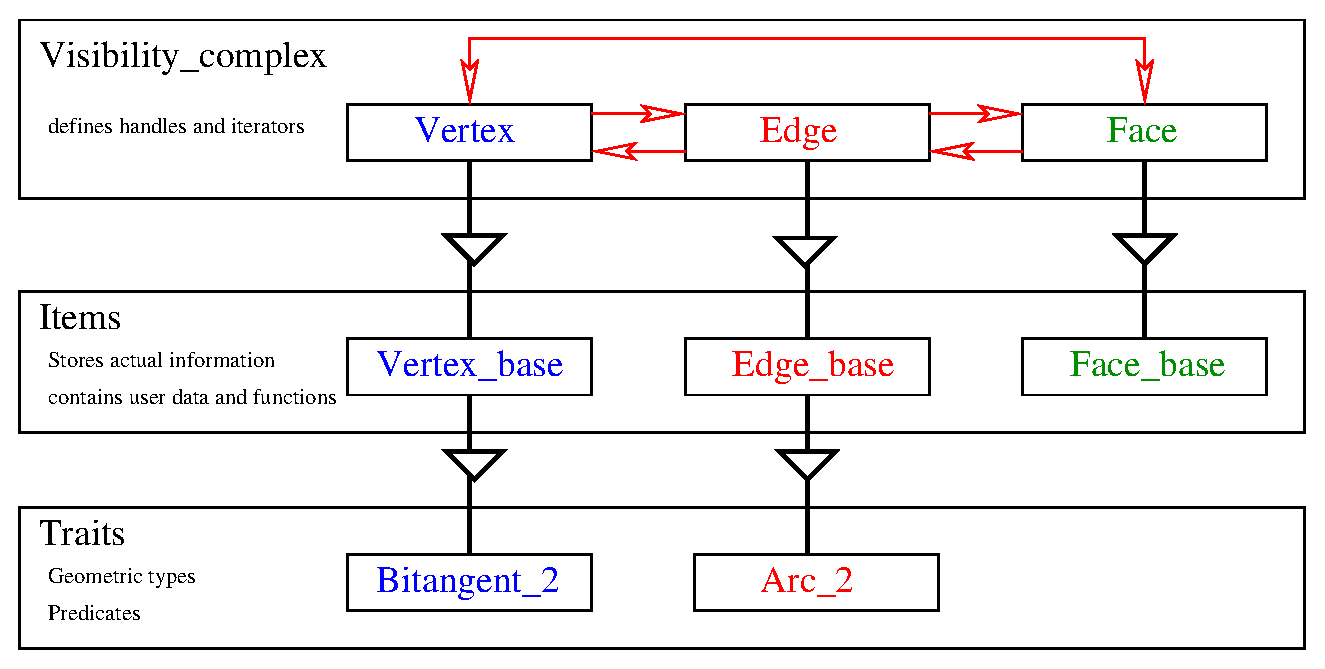
\includegraphics[width=0.7\textwidth]{fig/design.eps}%
      }
    \end{center}
    \caption{Three layer design of the visibility complex.}
    \label{figureVisibilityComplexDesign}
  \end{figure}
\end{ccTexOnly}

\begin{ccHtmlOnly}
    <CENTER>
    <A NAME="figureVisibilityComplexDesign">
        <img src="fig/design.gif"
         alt="Visibility Complex Design"><BR>
    Figure: Three layer design of the visibility complex.
    <P>
    </CENTER>
\end{ccHtmlOnly}

Figure~\ccTexHtml{\ref{figureVisibilityComplexDesign}}{}
\begin{ccHtmlOnly}
  <A HREF="Chapter_main.html#figureVisibilityComplexDesign"><IMG
  SRC="cc_ref_up_arrow.gif" ALT="reference arrow" WIDTH="10" HEIGHT="10"></A>
\end{ccHtmlOnly}
illustrates the responsibilities of the three layers of the software design.
The bottom layer is the geometric traits class \ccc{Traits} which defines the
geometric types (bitangents disks and arcs) and the predicates used to compute
the visibility complex. Currently four different traits classes are provided:
\begin{itemize}
    \item \ccc{Visibility_complex_point_traits<R>} for use with
    \ccc{CGAL::Point_2}.
    \item \ccc{Visibility_complex_circle_traits<R>} for use with
    \ccc{CGAL::Circle_by_radius_2}. The class \ccc{CGAL::Circle_by_radius_2}
    inherits from \ccc{CGAL::Circle_2} and is implemented in the file: 
    \begin{quote}
	\ccInclude{CGAL/Circle_by_radius_2.h}
    \end{quote}
    This class adds functionality to manipulate circles with their \emph{radius}
    instead of their \emph{squared radius}. 
    \item \ccc{Visibility_complex_segment_traits<R>} for use with
    \ccc{CGAL::Segment_2}.
    \item \ccc{Visibility_complex_polygon_traits<R>} for use with
    \ccc{CGAL::Polygon_2}.
\end{itemize}
The next layer is the \ccc{Items} class who defines, as local types, the
elements of the visibility complex. The user can enrich those classes by adding
his own data and member functions. The design used here is the same one used by
the \ccc{HalfedgeDS} in chapter~\ref{chapterHalfedgeDS}.

The two classes \ccc{Traits} and \ccc{Items} are passed as template parameters
to the class \ccc{Visibility_complex<Traits,Items>} who implements the
visibility complex structure. This former class defines the handle types which
are used to code the incidences between vertices, edges and faces. 

The visibility complex structure provides three pairs of iterators to traverse
its set of vertices, edges and faces. These are ordered as a linear extension of
a certain partial order $\prec$. See the last paragraph in
section~\ref{sectionVComplexInputOutput}.
% +============================================================================+
\section{Example Programs}
% +============================================================================+
\label{sectionVComplexExamples}

\subsection{Visibility complex of circles}
The following program reads a family of pairwise disjoint circles from the file
"input" and outputs the number of vertices in the visibility complex.

\ccIncludeExampleCode{Visibility_complex/vc_circle.C}

\subsection{Extending Faces}
The following example adds a \ccc{size} member variable to count the size of the
face. We use the \ccc{Antichain} to sweep the visibility complex while using
only $O(n)$ storage. The disks are of type \ccc{CGAL::Segment\_2} and $n$ is the
number of them.

\ccIncludeExampleCode{Visibility_complex/vc_face_extension.C}

% +----------------------------------------------------------------------------+

% EOF
